\section{操作指南}

按一场标准演出从开机到收尾的顺序写;路演 / 排练时按本节顺序走一遍,演出当天大概率不会卡。

\subsection{演出前 1 小时 · 准备}

\begin{enumerate}
  \item \textbf{装机}:在导播工作机(Windows 10/11)上运行 \texttt{StageDeck Remote\_v\sdVersion\_x64-setup.exe},一路下一步;预先装好 PowerPoint 365 / 2019,COM 接口要在。
  \item \textbf{准备 PPT}:打开演出用的 \texttt{.pptm}(若含答题/投票宏)或 \texttt{.pptx}(普通幻灯片)。进入幻灯片播放模式(F5 / Shift+F5),否则\,\app\ 抓不到\,\texttt{SlideShowWindow}。
  \item \textbf{打开\,\app}:从桌面快捷方式启动。看到导播 GUI 左侧"窗口选择"列表 —— 选中那个标着\,$\bigstar$\,的 PowerPoint 幻灯片放映窗(\app\ 已经按"演示窗优先"排好序)。
  \item \textbf{核对网络}:导播 GUI 顶部状态栏会显示 LAN 监听地址(\texttt{http://192.168.x.x:8787})和 Relay 状态(若已配置)。用自己手机扫一下 QR 码,确认能打开主持人页。能打开就回到导播,不打开就先排查 WiFi。
\end{enumerate}

\subsection{演出前 5 分钟 · 交接}

\begin{enumerate}
  \item \textbf{主持人扫码}:把手机递给主持人,扫导播 GUI 上的 QR(LAN 或 Relay 的二维码可在 GUI 切换)。主持人看到主持人页 —— 顶部大字"SLIDE \texttt{<n>}",底部一个全宽"下一页"按钮,中间一排 ARM / 黑屏 / 公告等操作。
  \item \textbf{开远控}:导播在 GUI 上把"远程控制"开关从 OFF 推到 ON。这一步之后,主持人页上的 ARM 按钮才能按。
  \item \textbf{主持人 ARM}:主持人在自己手机上点 ARM,顶部状态条变绿。此刻起主持人按"下一页"会真翻页。
  \item \textbf{走一遍预演}:翻 1-2 页测试反应;若 PPT 上有互动按钮,主持人页会自动出现对应的大按钮,选一个点一下验证宏触发。
\end{enumerate}

\begin{infobox}
\textbf{常见问题}:主持人扫码进去看到"未授权"或"401"。原因 99\% 是 token 过期(导播重启过 / 改过端口)。让导播在 GUI 里点"重置访问码",主持人重新扫一次新码即可。
\end{infobox}

\subsection{演出中 · 翻页 / 互动 / 急停}

\subsubsection*{翻页(最常用)}

\begin{itemize}
  \item 主持人手机底部全屏\textbf{下一页}按钮 —— 单手大拇指能按到。
  \item 上方有小按钮"上一页"。
  \item 导播 GUI 也能本地翻(用于"主持人手机意外离手"等兜底)。
\end{itemize}

\subsubsection*{触发 PPT 内嵌动作}

主持人页中间会自动显示当前幻灯片上所有带 VBA 宏绑定的形状(比如\,\kbd{选项 A}\,\kbd{选项 B}\,\kbd{公布答案})。点哪个就触发哪个,2 列大按钮排好,适合台上单手单触。

\subsubsection*{黑屏 / 恢复}

\begin{itemize}
  \item 主持人页\,\kbd{黑屏}\,—— 调 PowerPoint 的\,\texttt{BlackOut};
  \item 主持人页\,\kbd{恢复}\,—— 调\,\texttt{NormalView}。
  \item 适合节目交接、灯光秀间隙、临时中断。
\end{itemize}

\subsubsection*{紧急锁 —— 导播专用}

按一下:

\begin{enumerate}
  \item 主持人 ARM 立刻被清,主持人界面顶部条变红"已锁";
  \item 所有 \texttt{/api/next}, \texttt{/api/prev}, \texttt{/api/action} 之类的请求当场被服务端 403;
  \item 主持人不能自己再 ARM 回来 —— 必须导播先松锁,主持人再 ARM。
\end{enumerate}

适合:主持人下台 / 设备脱手 / 即将进入下个节目串场前的安全锁定。

\begin{center}
  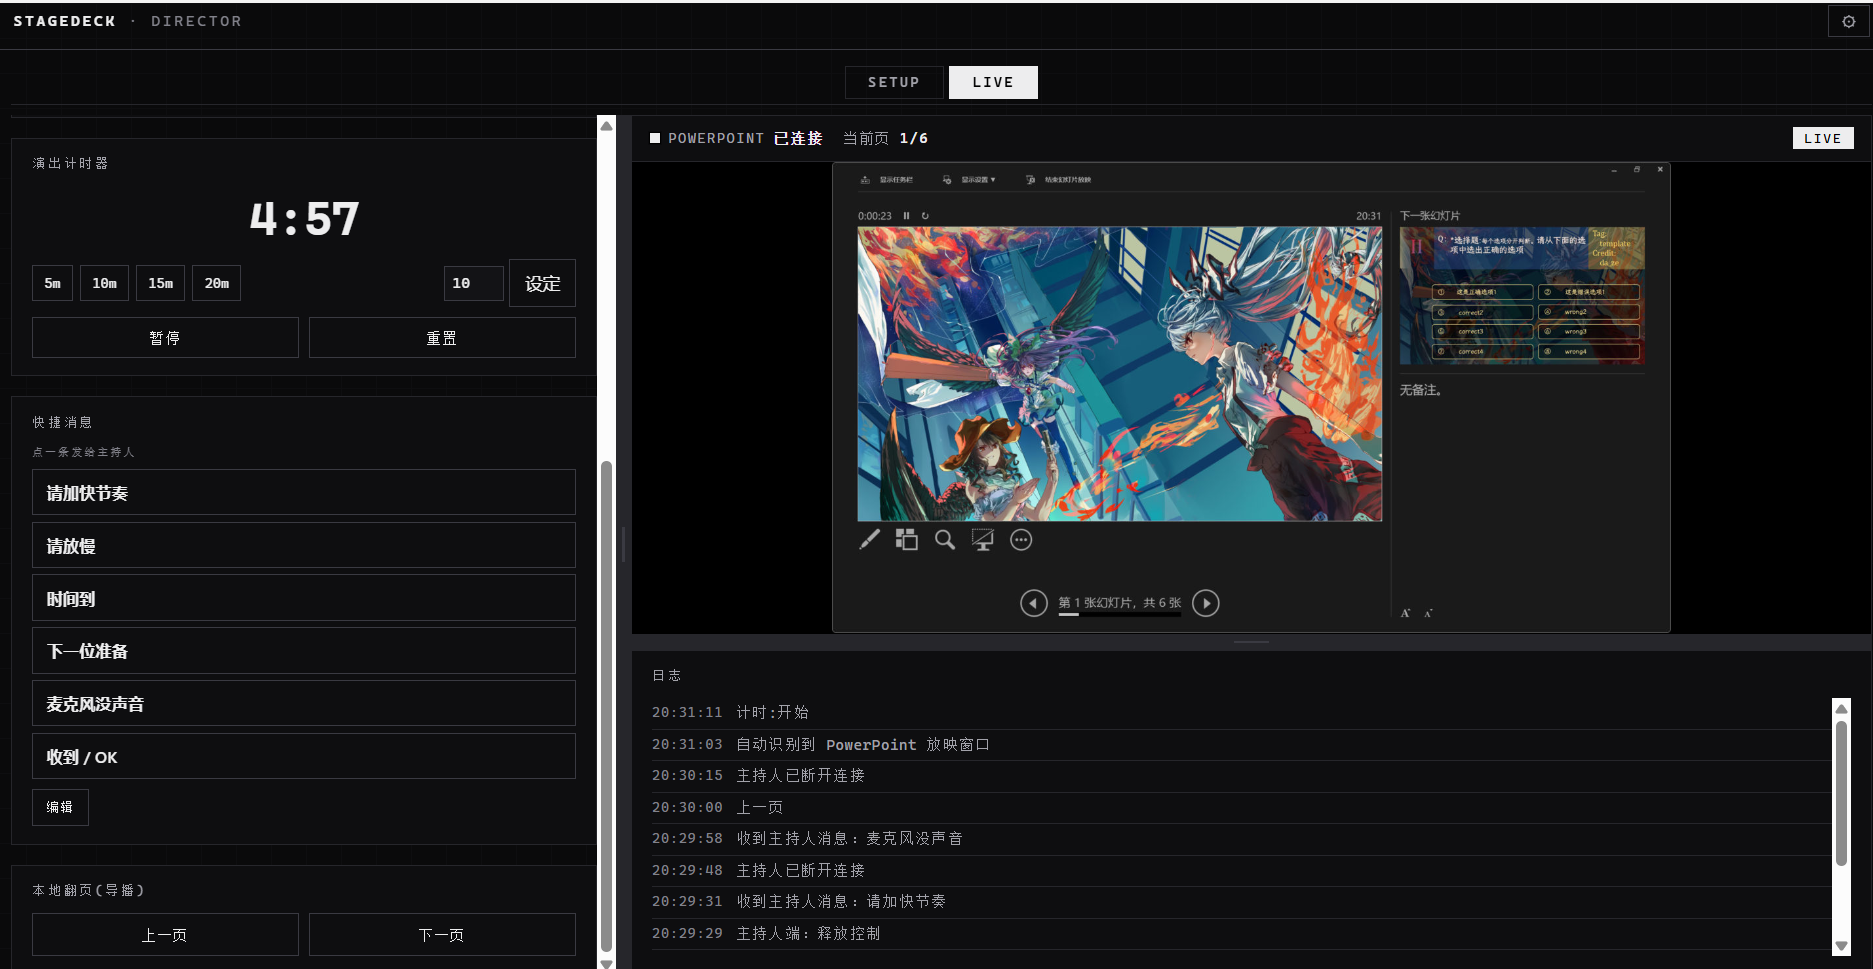
\includegraphics[width=\linewidth]{figures/example-pc.png}\\[3pt]
  {\small\sffamily\color{sddim} 导播 GUI 演出进行中 · Live 模式 · 顶部计时器倒数 / 快捷消息发布 / PPT 预览 + 日志 / 紧急锁底部待命}
\end{center}

\begin{center}
  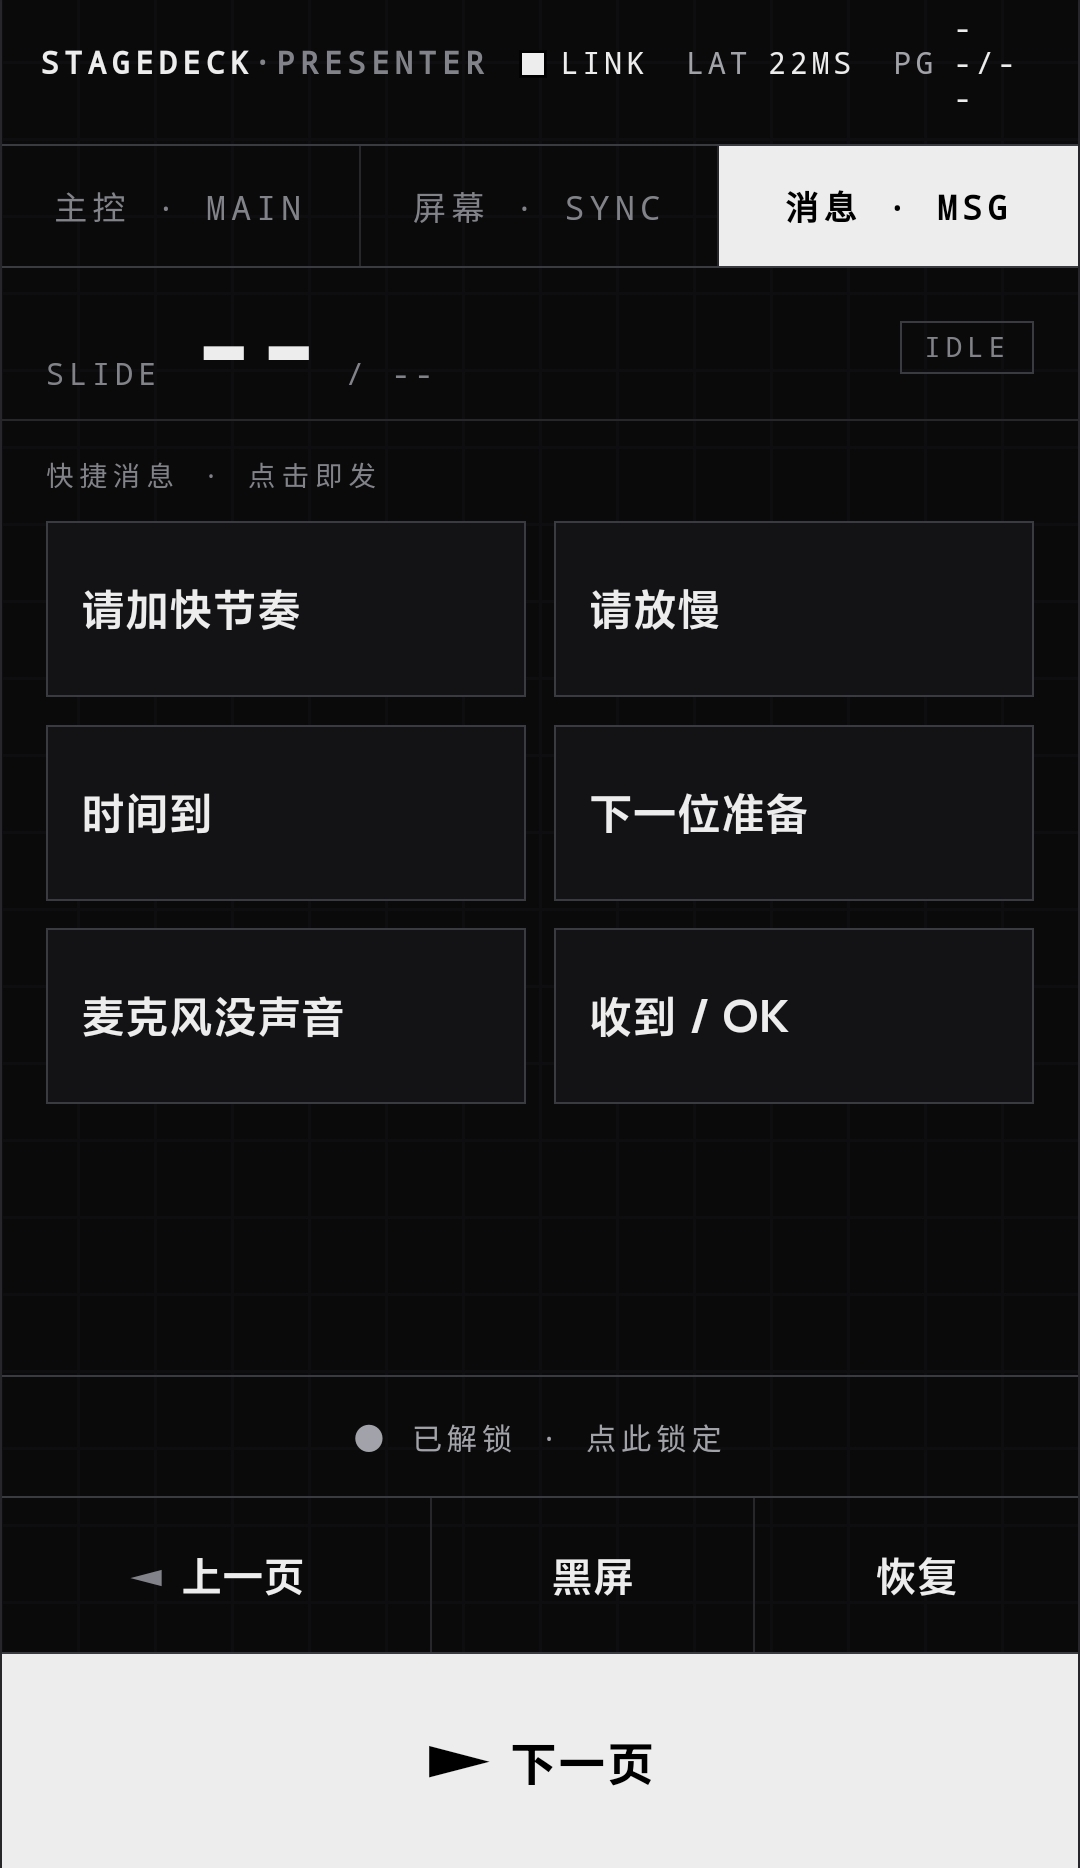
\includegraphics[height=240pt]{figures/example-android.jpg}\\[3pt]
  {\small\sffamily\color{sddim} 主持人手机 · 消息 tab · 6 个快捷消息大按钮 + 底部翻页全宽大按钮 + 顶部 LINK / LAT 22ms 状态条}
\end{center}

\subsection{演出后 · 收尾}

\begin{enumerate}
  \item 导播 GUI 关"远程控制"开关 —— 主持人页所有操作立刻失效。
  \item 退出\,\app\ —— Relay 隧道、本地 8787 监听全释放。
  \item 主持人不需要"退出"什么,关掉浏览器即可;下次演出新主持人重新扫码就是新会话。
\end{enumerate}

\subsection{排练 / 故障预案}

\begin{center}\small
\begin{tabularx}{\linewidth}{l X}
\toprule
\textbf{症状} & \textbf{处置}\\
\midrule
主持人页打不开 & 先确认手机和导播机在同一 WiFi;再确认导播 GUI 状态栏 LAN 地址正常;实在不行切 Relay 二维码。\\
扫码进去 401 / 拒绝 & 导播 GUI 点"重置访问码",主持人重新扫。\\
按下"下一页"没反应 & 检查导播 GUI 三件套:远控开?紧急锁松?主持人页顶部 ARM 绿?三选一关上就会失效。\\
画面卡住 & 检查 PowerPoint 是否仍在放映模式(F5);切出去再切回来\,\app\ 会重新抓窗。\\
PPT 互动按钮没出现 & 当前幻灯片上要有绑定 \texttt{ppMouseClick → ppActionRunMacro} 的形状;否则中间区域会空着,这是正常的。\\
Relay 状态红灯 & 校园网偶发抖动,自动重连 2-5 秒;若持续红,先切回 LAN 二维码再排查 Relay。\\
\bottomrule
\end{tabularx}
\end{center}
